\documentclass[10pt]{beamer}
\usepackage{amsmath}
\usepackage{mathtools}
\usefonttheme{professionalfonts} % using non standard fonts for beamer
\usefonttheme{serif} % default family is serif

%\documentclass[12pt]{beamerthemeSam.sty}
\usepackage{epsf}
%\usepackage{pstricks}
%\usepackage[orientation=portrait,size=A4]{beamerposter}
\geometry{paperwidth=160mm,paperheight=120mm}
%DT favorite definitions
\def\LL{\left\langle}	% left angle bracket
\def\RR{\right\rangle}	% right angle bracket
\def\LP{\left(}		% left parenthesis
\def\RP{\right)}	% right parenthesis
\def\LB{\left\{}	% left curly bracket
\def\RB{\right\}}	% right curly bracket
\def\PAR#1#2{ {{\partial #1}\over{\partial #2}} }
\def\PARTWO#1#2{ {{\partial^2 #1}\over{\partial #2}^2} }
\def\PARTWOMIX#1#2#3{ {{\partial^2 #1}\over{\partial #2 \partial #3}} }

\def\rightpartial{{\overrightarrow\partial}}
\def\leftpartial{{\overleftarrow\partial}}
\def\diffpartial{\buildrel\leftrightarrow\over\partial}

\def\BI{\begin{itemize}}
\def\EI{\end{itemize}}
\def\BE{\begin{displaymath}}
\def\EE{\end{displaymath}}
\def\BEA{\begin{eqnarray*}}
\def\EEA{\end{eqnarray*}}
\def\BNEA{\begin{eqnarray}}
\def\ENEA{\end{eqnarray}}
\def\EL{\nonumber\\}


\newcommand{\map}[1]{\frame{\frametitle{\textbf{Course map}}
\centerline{\includegraphics[height=0.86\paperheight]{../../map/#1.png}}}}
\newcommand{\wmap}[1]{\frame{\frametitle{\textbf{Course map}}
\centerline{\includegraphics[width=0.96\paperwidth]{../../map/#1.png}}}}

\newcommand{\etal}{{\it et al.}}
\newcommand{\gbeta}{6/g^2}
\newcommand{\la}[1]{\label{#1}}
\newcommand{\ie}{{\em i.e.\ }}
\newcommand{\eg}{{\em e.\,g.\ }}
\newcommand{\cf}{cf.\ }
\newcommand{\etc}{etc.\ }
\newcommand{\atantwo}{{\rm atan2}}
\newcommand{\Tr}{{\rm Tr}}
\newcommand{\dt}{\Delta t}
\newcommand{\op}{{\cal O}}
\newcommand{\msbar}{{\overline{\rm MS}}}
\def\chpt{\raise0.4ex\hbox{$\chi$}PT}
\def\schpt{S\raise0.4ex\hbox{$\chi$}PT}
\def\MeV{{\rm Me\!V}}
\def\GeV{{\rm Ge\!V}}

%AB: my color definitions
%\definecolor{mygarnet}{rgb}{0.445,0.184,0.215}
%\definecolor{mygold}{rgb}{0.848,0.848,0.098}
%\definecolor{myg2g}{rgb}{0.647,0.316,0.157}
\definecolor{abtitlecolor}{rgb}{0.0,0.255,0.494}
\definecolor{absecondarycolor}{rgb}{0.0,0.416,0.804}
\definecolor{abprimarycolor}{rgb}{1.0,0.686,0.0}
\definecolor{Red}           {cmyk}{0,1,1,0}
\definecolor{Grey}           {cmyk}{.7,.7,.7,0}
\definecolor{Blue}          {cmyk}{1,1,0,0}
\definecolor{Green}         {cmyk}{1,0,1,0}
\definecolor{Brown}         {cmyk}{0,0.81,1,0.60}
\definecolor{Black}         {cmyk}{0,0,0,1}

\usetheme{Madrid}


%AB: redefinition of beamer colors
%\setbeamercolor{palette tertiary}{fg=white,bg=mygarnet}
%\setbeamercolor{palette secondary}{fg=white,bg=myg2g}
%\setbeamercolor{palette primary}{fg=black,bg=mygold}
\setbeamercolor{title}{fg=abtitlecolor}
\setbeamercolor{frametitle}{fg=abtitlecolor}
\setbeamercolor{palette tertiary}{fg=white,bg=abtitlecolor}
\setbeamercolor{palette secondary}{fg=white,bg=absecondarycolor}
\setbeamercolor{palette primary}{fg=black,bg=abprimarycolor}
\setbeamercolor{structure}{fg=abtitlecolor}

\definecolor{A}{rgb}{1.0,0.0,0.0}
\definecolor{B}{rgb}{0.0,0.7,0.0}
\definecolor{C}{rgb}{0.7,0.7,0.0}
\definecolor{D}{rgb}{0.0,0.0,0.7}
\definecolor{E}{rgb}{0.4,0.4,0.4}

\setbeamerfont{section in toc}{series=\bfseries}

%AB: remove navigation icons
\beamertemplatenavigationsymbolsempty
\title[Newton's Law of Motion]{
  \textbf {Newton's Law of Motion}\\
%\centerline{}
%\centering
%\vspace{-0.0in}
%\includegraphics[width=0.3\textwidth]{propvalues_0093.pdf}
%\vspace{-0.3in}\\
%\label{intrograph}
}

\author[W. Freeman] {Physics 211\\Syracuse University, Physics 211 Spring 2023\\Walter Freeman}

\date{\today}

\begin{document}

\frame{\titlepage}

\frame{\frametitle{\textbf{Announcements}}
\BI
\Large
\item{Homework 3 due next Wednesday (will be posted today; shorter than HW2)}
\item{You will get new groups in recitation Friday or Wednesday}
\item{Exam 1 is mostly graded; you will get your grades back in recitation this week or next}
\EI

}
%
%\frame{\frametitle{\textbf{Exam 1}}
%\large
% \BI
%\item{Something was weird on Exam 1}
%\item{I may have to adjust the grading curve for the class, since the Physics Department standard for this class
%is that the average is a B-. Should I alter the syllabus to do that?}
% \EI
%\Large
%\bigskip
%\BI
%\item A: Yes
%\item B: No
%\pause
%\item C: Eh?
%\pause
%\item D: trollface.jpg?
%\EI
%}
%
%\frame{\frametitle{\textbf{Exam 1}}
%
%\large
%I showed my exam to my GTA's, some of whom have taught with me before. They said that it was moderately
%more challenging than last year's exam.
%
%\pause\bigskip
%
%I showed it to Julian Georg, who is the TA for Physics 215, the honors/majors version of my class. He showed me 
%the 215 exam, and said that ours was somewhat more difficult. 
%
%\pause\bigskip
%
%Of the exam grades I have so far, I have:
%
%\BI
%\item 70 F's
%\item 27 D's
%\pause
%\item 61 C's
%\pause
%\item 90 B's
%\pause
%\item \bf 202 A's
%\EI
%\pause
%
%
%\begin{center}
%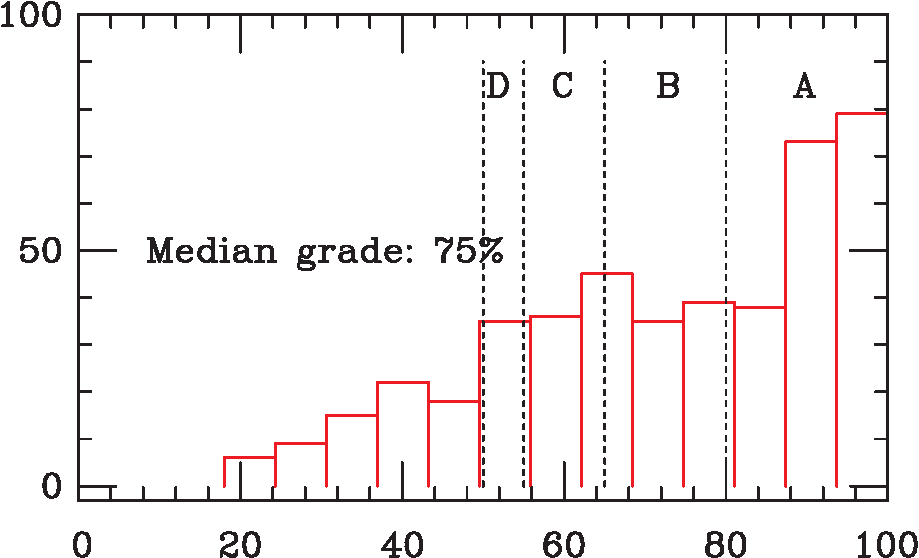
\includegraphics[width=0.5\textwidth]{gradehisto-crop.pdf}
%\end{center}
%
%}
%
%\frame{
%
%\begin{center}
%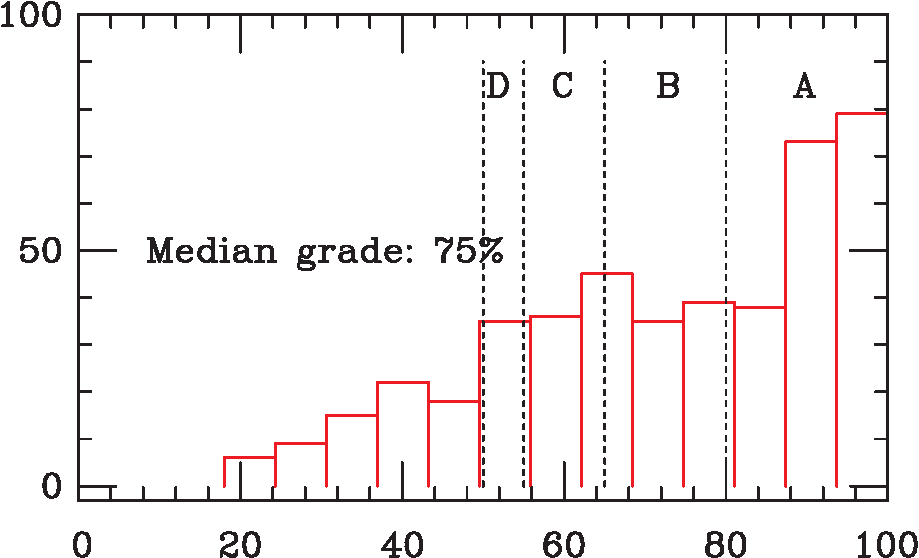
\includegraphics[width=0.5\textwidth]{gradehisto-crop.pdf}
%\end{center}
%
%\large
%
%Last year's exam had a median of 65\% (B-). That exam was perhaps a bit easier -- and had extra credit.
%
%\bigskip
%
%Your class median was {\bf 75\% (B+).} Be very, very proud of yourselves!
%}
%
%\frame{
%
%\Large
%
%Why do you think you did better than last year's class? (Seriously -- I'm curious to hear your guesses)
%
%\BI
%\item A: We're more motivated, smarter, or just overall more awesome than last year
%\item B: Group work in recitations / the group practice exam
%\item C: The physics practices on Wednesday evenings help
%\item D: The recitation TA's are a particularly good bunch
%\item E: This year's exam was easier
%\EI
%}

%\frame{\frametitle{\textbf{Ask a Physicist: general relativity and ``multiverses''}}
%
%}

\frame{\frametitle{\textbf{Newton's laws}}
    \Large

    \centerline{$\vec F = m\vec a$}
    \large
    \BI
  \item{Forces on an object cause it to accelerate}
  \item{The larger the force, the larger the acceleration}
  \item{The larger the mass, the smaller the acceleration}
  \item{You intuitively know this already}
    \pause
  \item{No forces $\rightarrow$ no acceleration: {\color{Red}not necessarily no motion!}}
    \bigskip
    \bigskip
\item{Forces come in pairs (Newton's third law)}
  \BI
\item{``If A pushes on B, B pushes back on A''}
\item{Very important to be clear about what forces you're talking about}
  \EI
    \EI
   }




   \frame{\frametitle{\textbf{Newtons}}
     \Large{\centerline{We need a new unit for force: the newton}}

     \bigskip
     \bigskip

     \centerline{     $\vec F = m \vec a \rightarrow$ Force has dimensions kg $\rm m/\rm s^2$}
\large
     \bigskip
     \bigskip
\BI
\item{1 N = 1 kg $\rm m/\rm s^2$: about the weight of an apple}

\item{4 N is about a pound}
     \item{9.8 N is the weight of a kilogram}
       \EI
   }

   \frame{\frametitle{\textbf{Force is a vector}}
     \Large
     \centerline{$\vec F = m\vec a$}
     \large
     \BI
   \item{Force is a {\it vector}}
   \item{Multiple forces on an object add like vectors do}
   \item{Really, we should write}
\EI
     \Large
     \centerline{$\sum \vec F = m\vec a$}


   }

   \frame{\frametitle{\textbf{What is a force?}}
    A force is anything that pushes or pulls something:
    \BI
  \item{Gravity: $F = mg$, so $mg = ma \rightarrow a = g$}
    \BI
  \item{Gravity pulls down on everything (on Earth) with a force $mg$, called its weight}
  \item{If something isn't accelerating downward, some other force must balance its weight}
  \item{We are now switching the way we think about gravity!}
  \BI
  \item Before: gravity makes objects in free fall accelerate downward at $g$
  \item Now: gravity is just one of {\it many} forces that can act on objects
  \EI
    \EI
    \EI
  }


  \frame{\frametitle{\textbf{What is a force?}}
    A force is anything that pushes or pulls something:
    \BI
  \item{Gravity: $F = mg$, so $mg = ma \rightarrow a = g$}
  \item{``Normal force'': stops things from moving through each other}
    \BI
  \item{Are there normal forces on me right now?}
 \pause
  \item{However big it needs to be to stop objects from sliding through each other}
  \item {\color{A}The normal force is usually an unknown you will need to solve for, not a thing you know}
  \item{Directed ``normal'' (perpendicular) to the surface}
  \item{Really caused by electric force/Pauli exclusion principle}
    \EI
    \EI
  }


  \frame{\frametitle{\textbf{What is a force?}}
    A force is anything that pushes or pulls something:
    \BI
  \item{Gravity: $F = mg$, so $mg = ma \rightarrow a = g$}
  \item{``Normal force'': stops things from moving through each other}
  \item{Tension: ropes pull on both sides equally}
%    \BI
%  \item{What are the forces on the people in a contest of tug-of-war?}
%
%  \pause
%    \EI
%  \item{Friction: a force opposes things sliding against each other {\color{D}(We'll learn about this next week)}}
    \pause
  \item{Electromagnetic forces, nuclear forces, radiation pressure...}
    \pause
  \item{\color{Red}Acceleration is not a force!}
  \item{\color{Red}... it's the {\it result} of forces}
    \EI
  }

\frame{\frametitle{\textbf{One particular force: gravity}}

\Large

Gravity exerts a downward force on all objects (on Earth), with a magnitude of $mg$.

\bigskip

In symbols: $\vec F_g = mg$ downward.

\bigskip
\pause

Why is the acceleration of a falling object $g$ downward?
 
\BI
\item \color{A}A: Because $g$ is the acceleration of all objects within Earth's gravitational field
\item \color{B}B: Solve Newton's law: $\vec F = m \vec a \rightarrow mg (-\hat j) = m\vec a \rightarrow \vec a = -g\hat j$
\item \color{C}C: Because the definition of $g$ is the acceleration that a falling object undergoes
\item \color{D}D: It's only $g$ if there are no other forces besides gravity acting on it\EI
} 



  \frame{\frametitle{\textbf{Force diagrams}}
  \BI
  \item{Lots of forces, easy to get confused}
  \item{Draw a picture!}
    \centerline{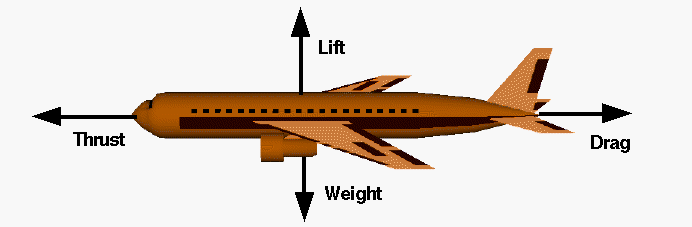
\includegraphics[width=0.6\textwidth]{cruise.png}}
    \pause
  \item{Each object feeling forces gets a separate diagram}
  \item{Label each force and its direction}
  \item{These are also called ``free body diagrams''}
    \EI
  \bigskip
  \bigskip
  \bigskip
  \bigskip
  \pause
  \small
  \centerline{(Examples on document camera)}

  }

\frame{\frametitle{\textbf{An example}}

(Use 10 $\rm m/\rm s^2$ for $g$, please!)

\bigskip

An aircraft at an air show has a mass of 10,000 kg and its engine produces a maximum thrust of 130 kN.

\bigskip

If it is using its engine at full power to take off (on the ground), what is its acceleration?

\bigskip

(Neglect air resistance for now -- this only matters once it is moving quickly)

\Large



\BI
\item \color{A}A: 10 $\rm m/\rm s^2$ downward
\item \color{B}B: 13 $\rm m/\rm s^2$ forward
\item \color{C}C: 23 $\rm m/\rm s^2$ forward
\item \color{D}D: 3 $\rm m/\rm s^2$ forward
\EI

}

\frame{\frametitle{\textbf{An example}}

The pilot wants to show off for the crowd, so they point the aircraft straight upward once it is in the air.

\bigskip

	(Again, it has a mass of 10,000 kg and its engine has a thrust of 130 kN.)
	
	\bigskip
	
	
	
	What is its acceleration now?
	
	\Large
	
	\BI
	\item \color{A}A: 10 $\rm m/\rm s^2$ downward
	\item \color{B}B: 3 $\rm m/\rm s^2$ downward
	\item \color{C}C: 13 $\rm m/\rm s^2$ upward
	\item \color{D}D: 3 $\rm m/\rm s^2$ upward
	\item \color{E}E: 23 $\rm m/\rm s^2$ upward
	\EI
	
}


\frame{\frametitle{\textbf{An example}}
	
	Suppose the pilot then dives straight down at high speed, using their engines to push them downward faster.
	
	\bigskip
	
	Since they are going so fast, there is substantial air resistance.
	
	\bigskip
	
	If the plane's acceleration is 8 $\rm m/\rm s^2$ downward, what is the force of air resistance? 	(Again, the aircraft has a mass of 10,000 kg and its engine has a thrust of 130 kN.)
	
	\Large
	
	\BI
	\item \color{A}A: 100 kN downward
	\item \color{B}B: 100 kN upward
	\item \color{C}C: 150 kN upward
	\item \color{D}D: 80 kN downward
	\item \color{E}E: 230 kN upward
	\EI
	
}



%\frame{\frametitle{\textbf{A sample problem}}
%	
%	\Large
%	
%	The people on the right cart pull on the people on the left cart. Suppose the acceleration of the left cart is $0.2\,\rm m/\rm s^2$.
%	
%	\bigskip
%	
%	What will the acceleration of the right cart be?
%	
%	\bigskip
%	\begin{itemize}
%
%
%\item \color{A}A: $0.2\,\rm m/\rm s^2$
%\item \color{B}B: $0.1\,\rm m/\rm s^2$
%\item \color{C}C: $0.4\,\rm m/\rm s^2$
%\item \color{D}D: 0
%\end{itemize}	
%}


\frame{
\large

Suppose an object is moving in a straight line at a constant speed. Which number of forces could {\it not} be 
acting on it?
\bigskip

\BI
\item \color{A}A: Zero
\item \color{B}B: One
\item \color{C}C: Two
\item \color{D}D: Three
\item \color{E}E: Four
\EI

\pause
\bigskip\bigskip
Suppose an object is moving in a circle at a constant speed. Which number of forces could {\it not} be 
acting on it? (Hint: what is the definition of velocity? Of acceleration?)
\bigskip

\BI
\item \color{A}A: Zero
\item \color{B}B: One
\item \color{C}C: Two
\item \color{D}D: Three
\item \color{E}E: Four
\EI
}


  \frame{\frametitle{\textbf{Sample questions}}
    \BI
    \Large
  \item{What forces act on a car?}
    \pause
  \item{Which forces are bigger or smaller if it's driving at a constant speed?}
    \pause
  \item{Which forces are bigger or smaller if it's slowing down?}
    \pause
  \item{A 1000 kg car slows from 20 m/s to a stop over 5 sec. What force is required to do this?}


    \pause

\bigskip
\bigskip
\bigskip
\normalsize
\centerline{(Use $\vec F = m \vec a$ to connect force to acceleration, and then kinematics to connect acceleration to motion)}

    \EI
  }

\frame{\frametitle{\textbf{An important note}}
\large
\BI
\item{Only {\it real physical things} are forces}
\pause
\item{Acceleration is not a force}
\item{``Net force'' is not a force (it's the sum of them)}
\item{Velocity certainly isn't a force}
\pause
\item{If two things don't touch, or interact by gravity, electricity, etc., they don't
exchange forces}
\pause
\item{``A force is something that can send you to the doctor''}
\EI
}



\frame{\frametitle{\textbf{A sample problem}}
\Large
A stack of two books sits on a table. Each book weighs 10 newtons. Draw a force diagram
for each one, and calculate the size of all the forces.

\bigskip
\bigskip
\bigskip

(Your answer should match what you know about how this works!)
}

\frame{
	\Large
	Which of the following is/are {\it not} an example of Newton's third law?
	
	\bigskip
	
	\BI
	\item \color{A}A: a subway car accelerates forward; you are thrown back
	\item \color{B}B: the propeller on an airplane pushes the air backwards; the air pushes the airplane forwards
	\item \color{C}C: an elevator accelerates upward; passengers are pushed downward
	\item \color{D}D: the Earth's gravity pulls downward on me; my gravity pulls upward on the Earth
	\item \color{E}E: a rocket pushes downward on its exhaust; the exhaust pushes upward on the rocket
	\EI}


  \frame{\frametitle{\textbf{Summary}}
    \Large
    \BI
  \item{Forces: anything that pushes or pulls}
  \item{Forces cause accelerations: $\sum \vec F = m \vec a$}
    \BI
  \item{If $\sum \vec F = 0$, $\vec a = 0$: motion at a constant velocity}
  \EI
  \item{Forces come in pairs: if A pushes on B, B pushes back on A}
  \item{It's the vector sum $\sum \vec F$ that matters}
  \item{Draw force diagrams to keep all of this straight}
    \EI
  }



  \end{document}

